
\vspace{0.5cm}

El siliceno hidrogenado es conocido como el silicio, tiene una estructura similar al siliceno pero 
con átomos de hidrógeno alternando en el plano formando una hibridación $sp^{3}$.

\vspace{0.5cm}

\begin{figure}[H]
    \centering
    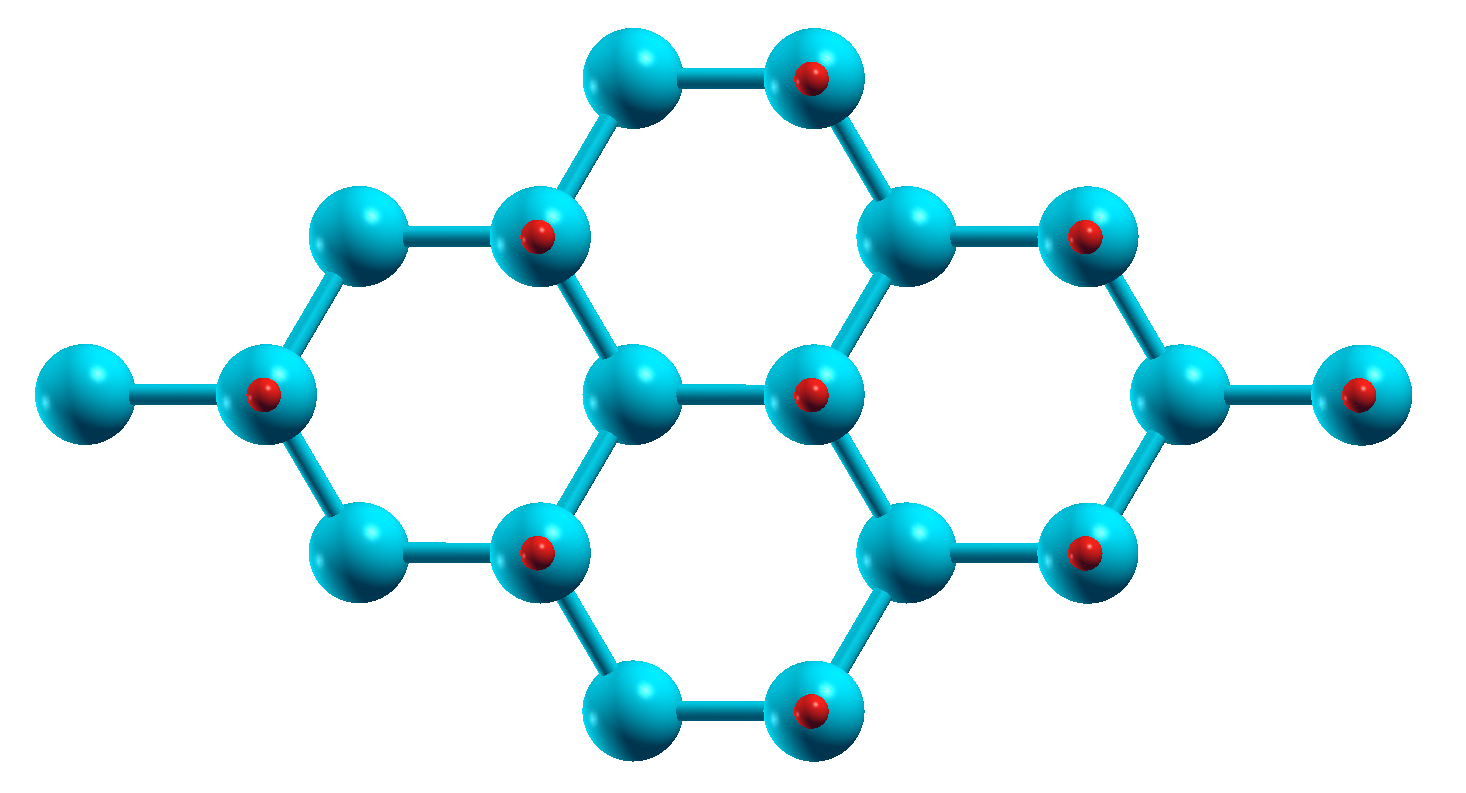
\includegraphics[scale=0.3]{images_silicano/silicano_structure.png}
    \caption{Estructura cristalina del Siliceno obtenida del archivo input con Xcrysden [Celda primitiva]}
\end{figure}

\vspace{0.5cm}

\begin{figure}[H]
    \centering
    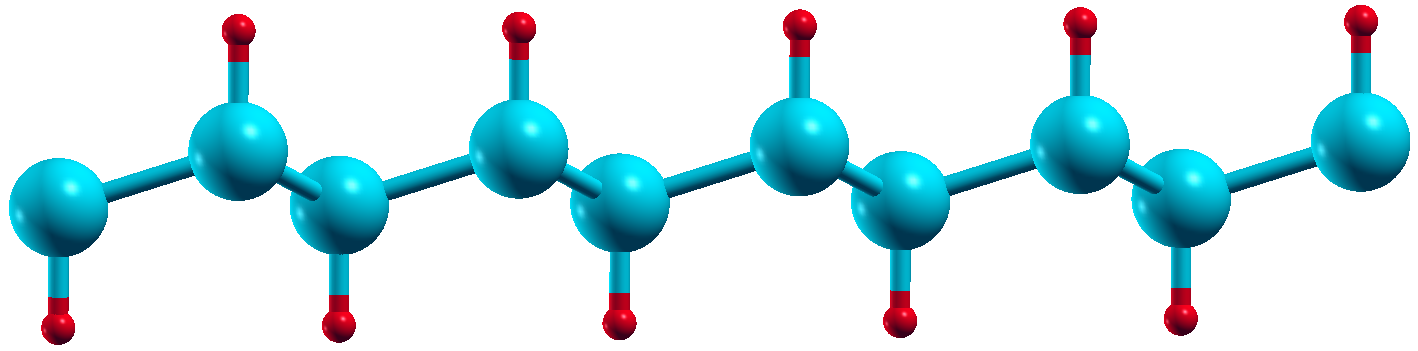
\includegraphics[scale=0.3]{images_silicano/silicano_structure_2.png}
    \caption{Estructura cristalina del Siliceno (otra perspectiva) [Celda primitiva]}
\end{figure}

\begin{table}[H]
    \begin{center}
        \begin{tabular}{| c | c |}
            \hline
            \multicolumn{2}{ |c| }{\textbf{Archivo inicial}} \\ \hline
            ibrav & 0 \\ \hline
            nat & 4 \\ \hline
            ntype & 2 \\ \hline
            occupations & smearing \\ \hline
            degauss & 0.01 \\ \hline
            smearing & 'm-p' \\ \hline
            Cell parameters  {alat}  & 0.500 0.866 0.000  \\
                                     & -0.500 0.866 0.000 \\
                                     & 0.000 0.000 5.144  \\ \hline
            Atomic Positions Crystal & H  0.000 0.000 0.000  \\
                                     & Si 0.000 0.000 0.075  \\
                                     & Si 0.333 0.333 0.111  \\
                                     & H  0.333 0.333 0.186 \\  \hline
        \end{tabular}
        \caption{Principales paramétros del silicano}
        \label{tab: Parametros del Silicano}
    \end{center}
\end{table}

A continuación, realizaremos los siguientes cálculos y optimizaciones:

\begin{itemize}
    \item Optimización Ecutwfc [Silicano]
    \item Optimización Ecutrho [Silicano]
    \item Optimización K-points [Silicano]
    \item Optimización Lattice parameter (parámetro de red) [Silicano]
    \item Cálculo de bandas [Silicano]
    \item Densidad de estados sin considerar el spin [Silicano]
    \item Densidad de estados considerando el spin [Silicano]
\end{itemize}


% Optimización Ecutwfc [Silicano]

\newpage

\subsection{Optimización Ecutwfc [Silicano]}

\vspace{0.5cm}

Buscamos obtener un valor mínimo para el parámetro Ecutwfc donde podamos observar 
que converge la energía de la estructura cristalina.

\vspace{0.5cm}

Vamos a variar el valor del paramétro Ecutwfc de 20 a 50 en pasos de 5 en 5, así realizaremos un cálculo de
SCF y un ploteo de Ecutwfc contra la energía total de la estructura.

\vspace{0.5cm}

\begin{figure}[H]
    \centering
    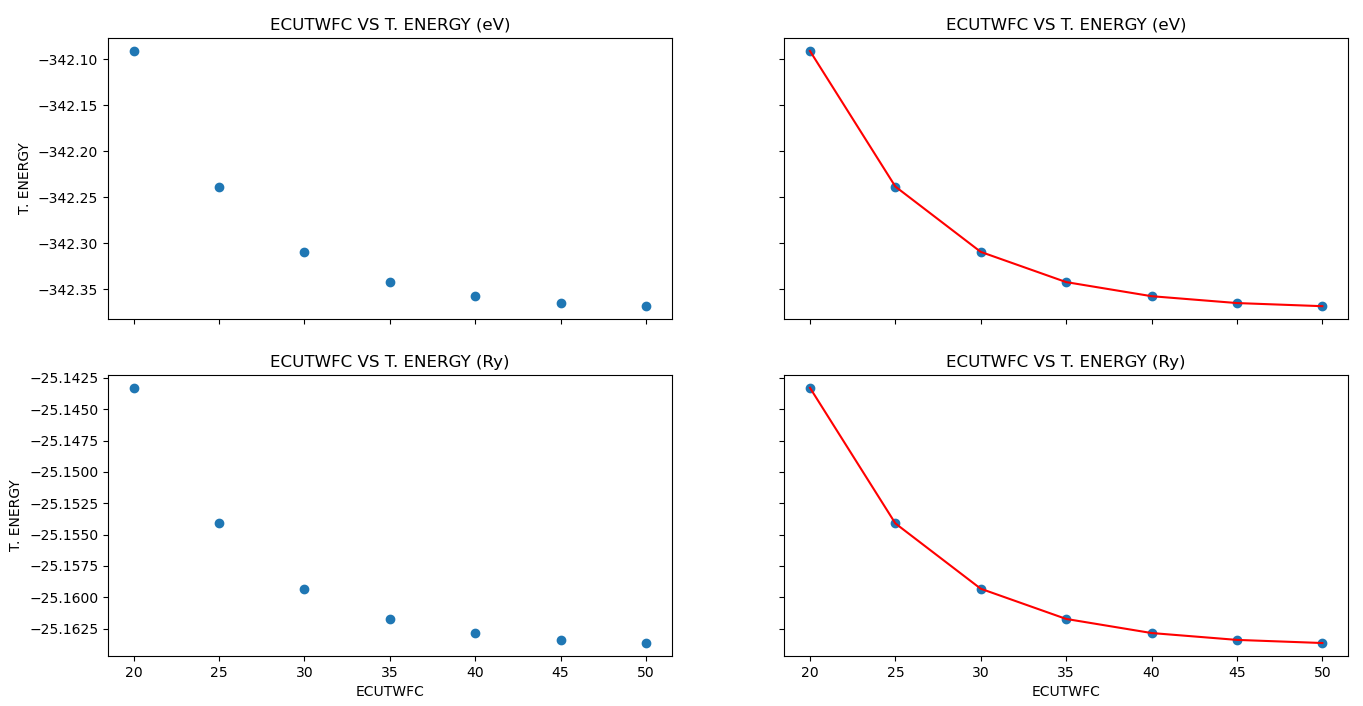
\includegraphics[scale=0.32]{images_silicano/Ecutwfc_vs_Energy.png}
    \caption{Gráfica que nos muestra la energía total del sistema contra la variación del parámetro ecutwfc.}
\end{figure}


Observación: el valor de la variable dependiente (la energía total) empieza su convergencia cuando 
la variable independiente (ecutwfc) empieza a tomar valores a partir de 35.


% Optimización Ecutrho [Silicano]

\newpage

\subsection{Optimización Ecutrho [Silicano]}

\vspace{0.5cm}

Ahora vamos a buscar optimizar el valor del paramétro Ecutrho, donde para fines de nuestra actividad 
supondremos que es un múltiplo de el valor que toma Ecutwfc, donde depende de la siguiente forma:

\begin{equation*}
    Ecutrho = k*Ecutwfc
\end{equation*}

Donde $ k \in \mathbb{N}  $

\vspace{0.5cm}

Buscamos obtener un valor mínimo para k de tal manera que podamos observar que la energía de la
estructura cristalina converge.

\vspace{0.5cm}

Vamos a variar el valor de k de 1 a 12 en pasos de 1 en 1, así realizaremos un cálculo de
SCF y un ploteo del valor de k contra la energía total de la estructura.

\begin{figure}[H]
    \centering
    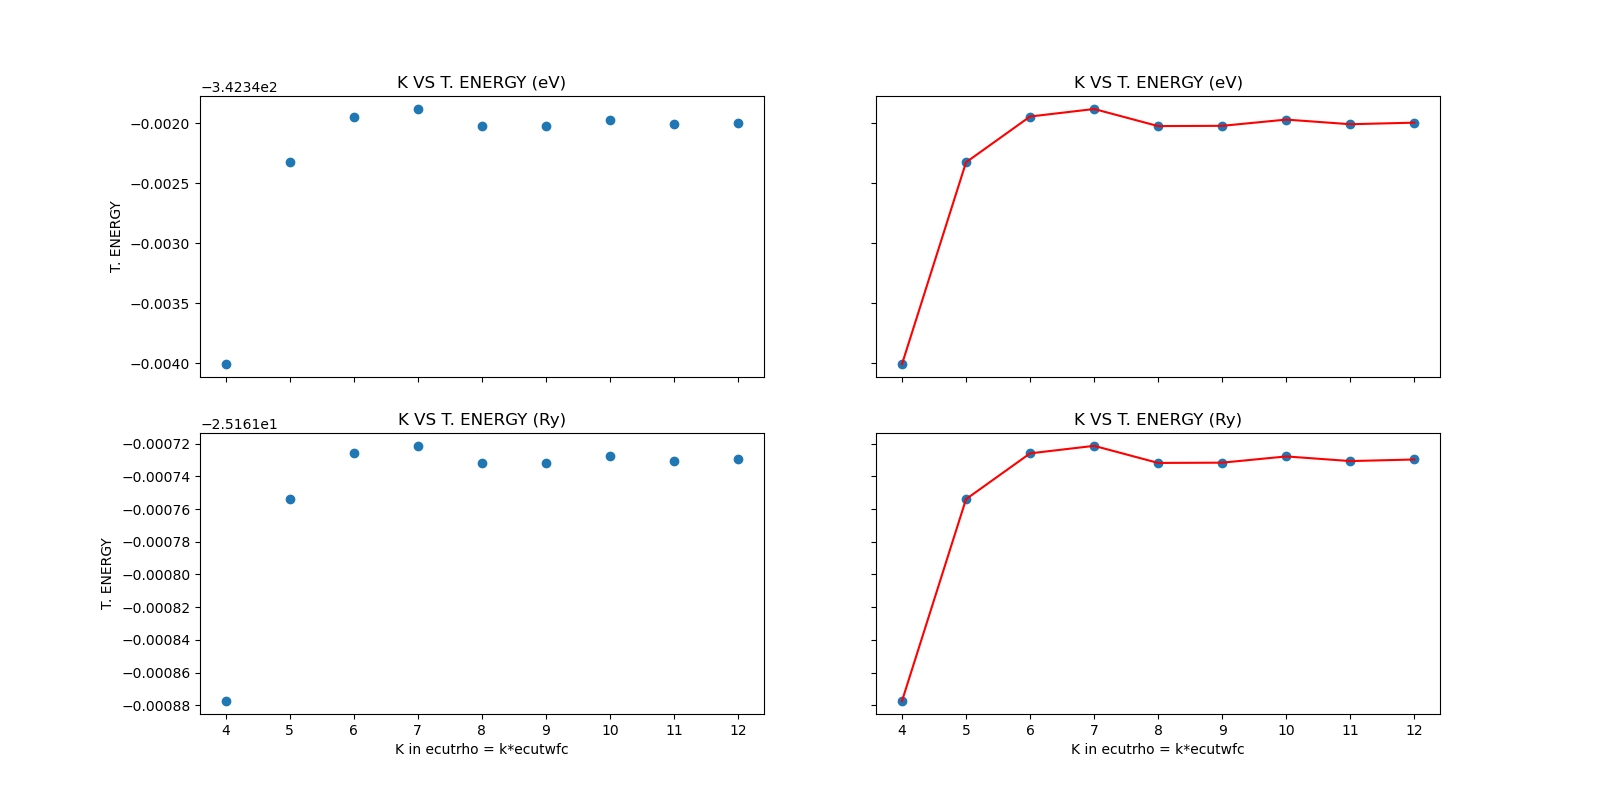
\includegraphics[scale=0.33]{images_silicano/K_in_ecutrho_vs_Energy.png}
    \caption{Gráfica que nos muestra la energía total del sistema contra la variación del parámetro k, nos centramos en el intervalo [4,12]}
\end{figure}

Observación: el valor de la variable dependiente (la energía total) empieza su convergencia cuando 
la variable independiente (ecutwfc) empieza a tomar valores a partir de 6.


% Optimización K-points [Silicano]

\newpage

\subsection{Optimización K-points [Silicano]}

\vspace{0.5cm}

A continuación realizaremos una optimización para los puntos K del silicano. En nuestro archivo input estos
tienen la forma de la siguiente expresión: 

\begin{equation*}
    i \; i \; 1 \; 0 \; 0 \; 0
\end{equation*}

Donde $ i \in \mathbb{N}  $ .

\vspace{0.5cm}

Buscamos obtener un valor mínimo para i de tal manera que podamos observar una convergencia en la 
energía del sistema.

\begin{figure}[H]
    \centering
    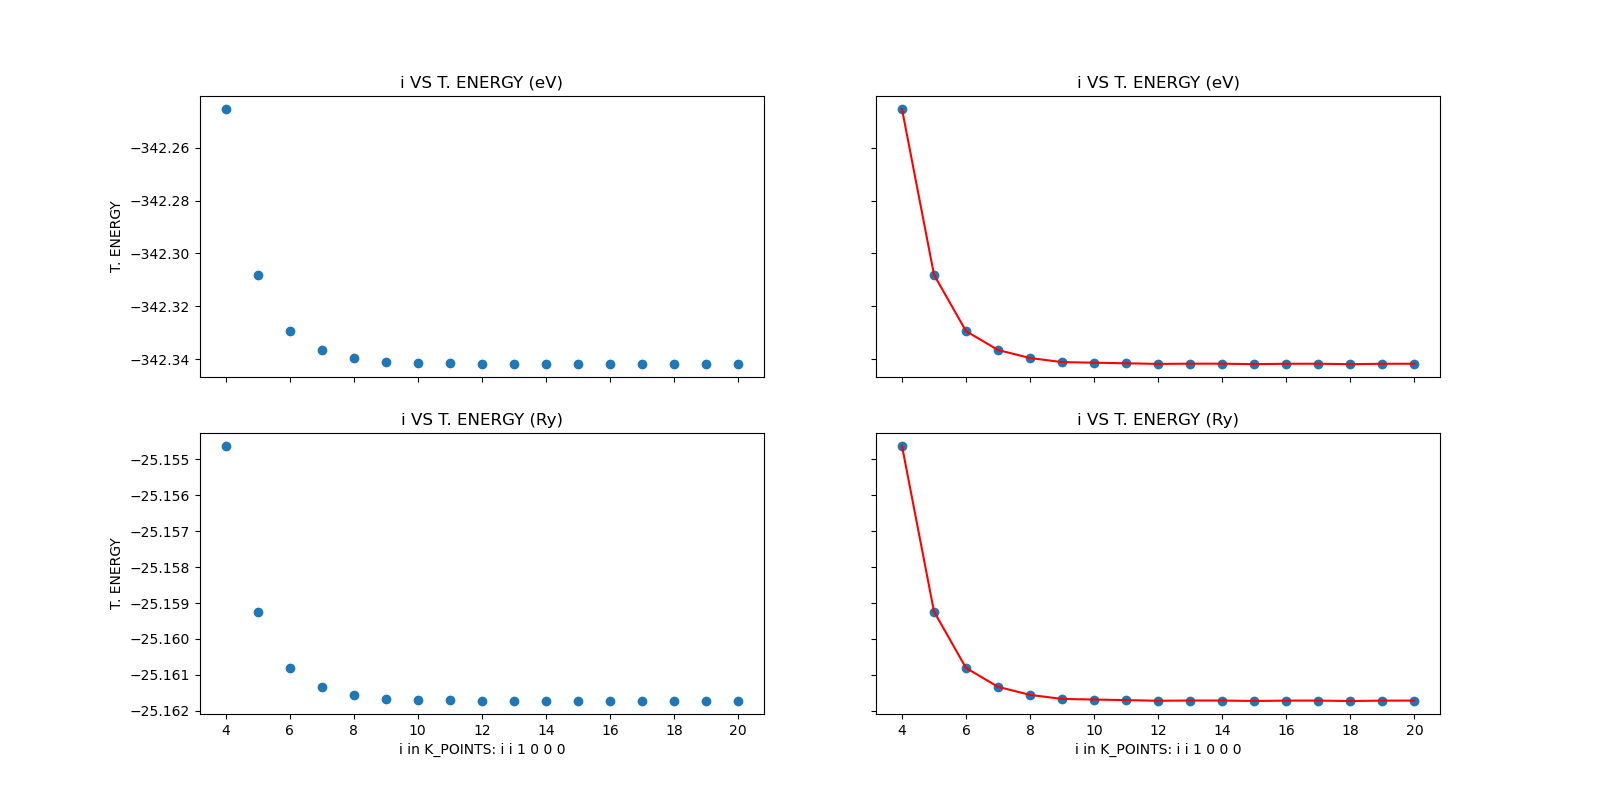
\includegraphics[scale=0.33]{images_silicano/K_points_vs_Energy.png}
    \caption{Gráfica que nos muestra la energía total del sistema contra la variación del parámetro k, nos centramos en el intervalo [4,12]}
\end{figure}

\vspace{0.5cm}

Observación: el valor de la variable dependiente (la energía total) empieza su convergencia cuando 
la variable independiente (i) empieza a tomar valores alrededor de 8.



% Optimización Lattice parameter (parámetro de red) [Silicano]

\newpage

\subsection{Optimización Lattice parameter (parámetro de red) [Silicano]}

\vspace{0.5cm}

Ahora vamos a buscar optimizar el valor del paramétro de red, haremos una inspección probando valores
en el siguiente intervalo [3.0, 5.0].
 
\vspace{0.5cm}

Buscamos obtener un valor mínimo para el paramétro de red de tal manera que podamos observar que la energía
de la estructura cristalina converge.

\vspace{0.5cm}

Empezaremos desde el 3.0 y para cada uno haremos un calculo del tipo "relax", repetiremos el proceso
en saltos de 0.1 en 0.1 hasta alcanzar el valor de 5.0.

\begin{figure}[H]
    \centering
    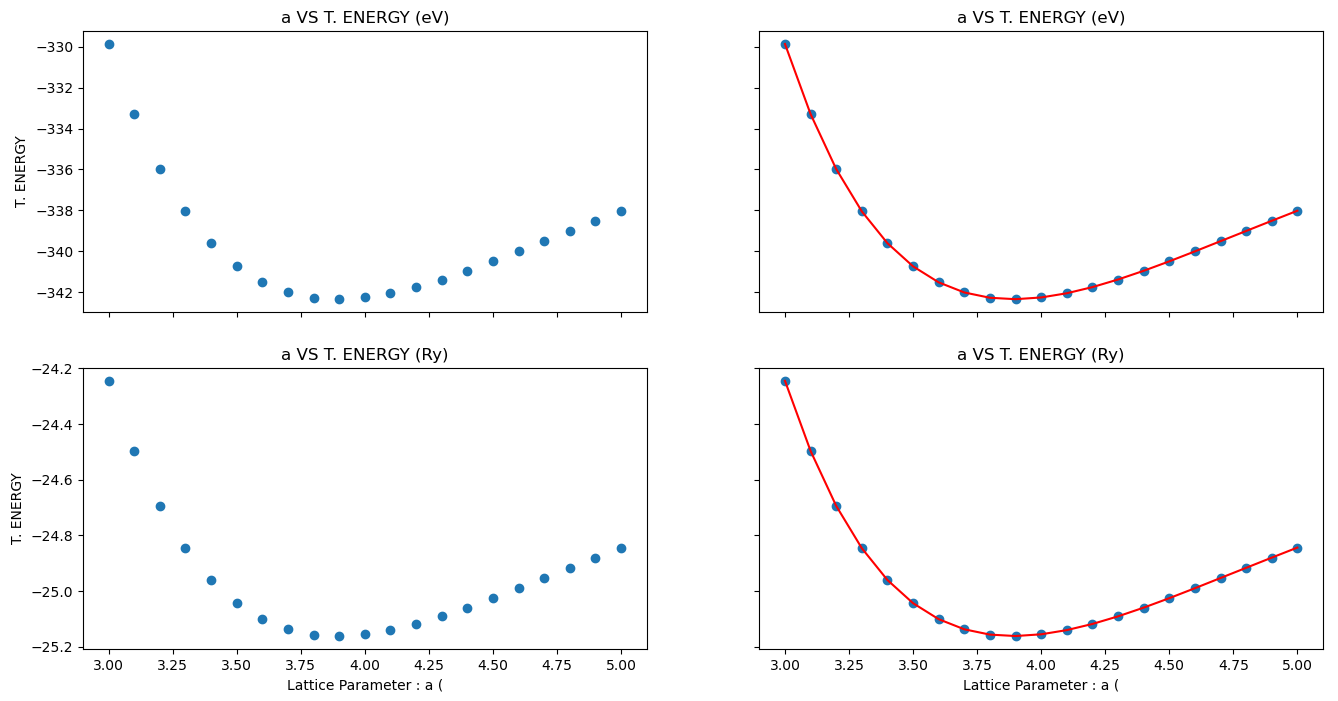
\includegraphics[scale=0.33]{images_silicano/Lattice_parameter_vs_Energy.png}
    \caption{Gráfica que nos muestra la energía total del sistema contra la variación del parámetro k, nos centramos en el intervalo [3.0, 5.0]}
\end{figure}

\vspace{0.5cm}

Observación: el valor de la variable dependiente (la energía total) empieza su convergencia cuando 
la variable independiente (paramétro de red) empieza a tomar valores cercanos a 3.9.


% Cálculo de bandas [Silicano]

\newpage

\subsection{Cálculo de bandas [Silicano]}

En el siguiente apartado damos una gráfica con la estructura electrónica de bandas del silicano. 
Para obtener esta estructura es necesario realizar la siguiente serie de cálculos.
Primero realizamos un cálculo con el módulo pw.x, después otro cálculo 
del tipo scf y por último uno del tipo bands. Se llegó al siguiente gráfico:

\begin{figure}[H]
    \centering
    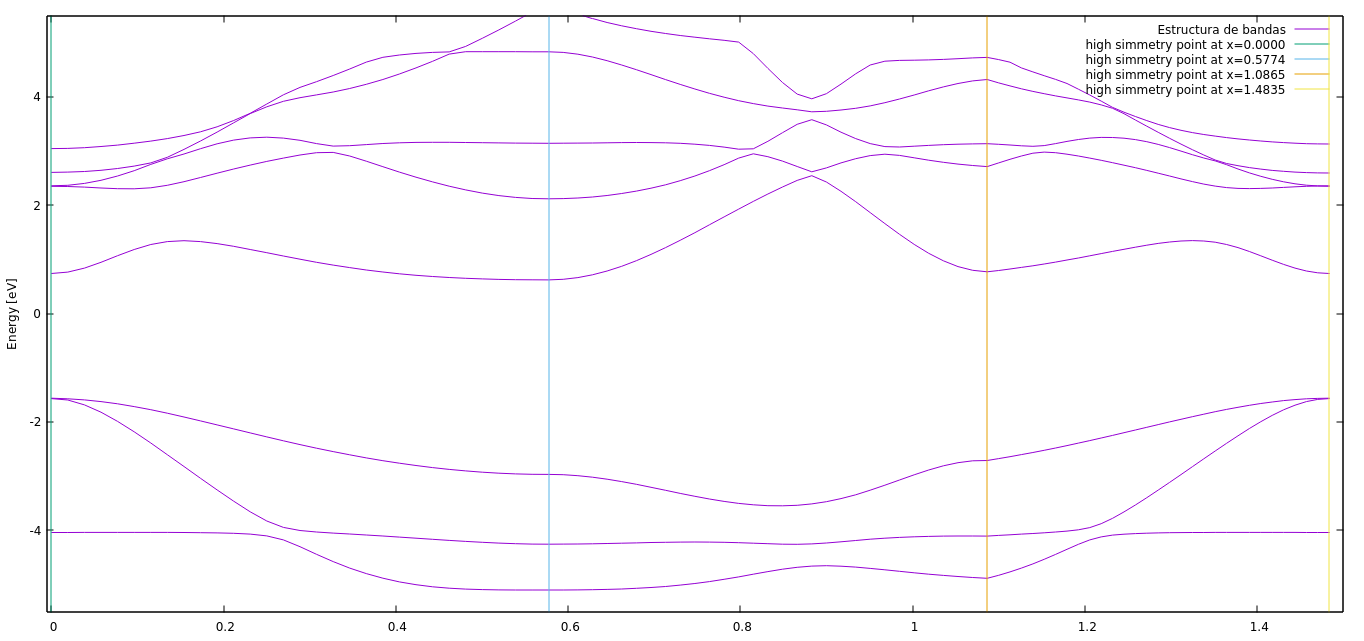
\includegraphics[scale=0.45]{images_silicano/bands_structure_silicane_10_bands_relax.png}
    \caption{Gráfica que nos muestra la estructura de bandas del siliceno, cuyo cálculo fue elaborado por cuenta propia}
\end{figure}

En la literatura podemos encontrar estructuras similares, como por ejemplo:

\begin{figure}[H]
    \centering
    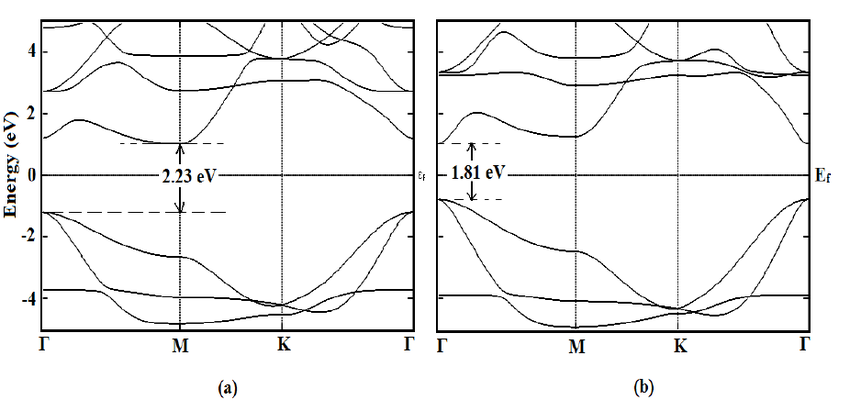
\includegraphics[scale=0.5]{images_silicano/Bandstructure-of-a-silicane-and-b-germanane.png}
    \caption{Gráfica que nos muestra la estructura de bandas del silicano [a)] \cite{trivedi2014silicene} }
\end{figure}

\vspace{0.2cm}

Observación: Ambas son semejantes. Se observan discrepencias,
sin embargo, cabe la posibilidad que sea debido al poder de computo del que se dispone.


% Densidad de estados sin considerar el spin [Silicano]

\newpage

\subsection{Densidad de estados sin considerar spin [Silicano]}

En el siguiente apartado damos una gráfica con la densidad de estados del siliceno. Para 
ello se hizo el cálculo dentro del mismo Quantum Espresso con el módulo pw.x, primero se hizo uno cálculo 
del tipo nscf y después otro del tipo DOS. También para este momento se trabajó con la estructura
ya relajada.

\vspace{0.5cm}

\textbf{Importante: En el siguiente cálculo no se consideró el spin.}

\vspace{0.5cm}

\vspace{0.5cm}

Se llegó al siguiente gráfico:

\begin{figure}[H]
    \centering
    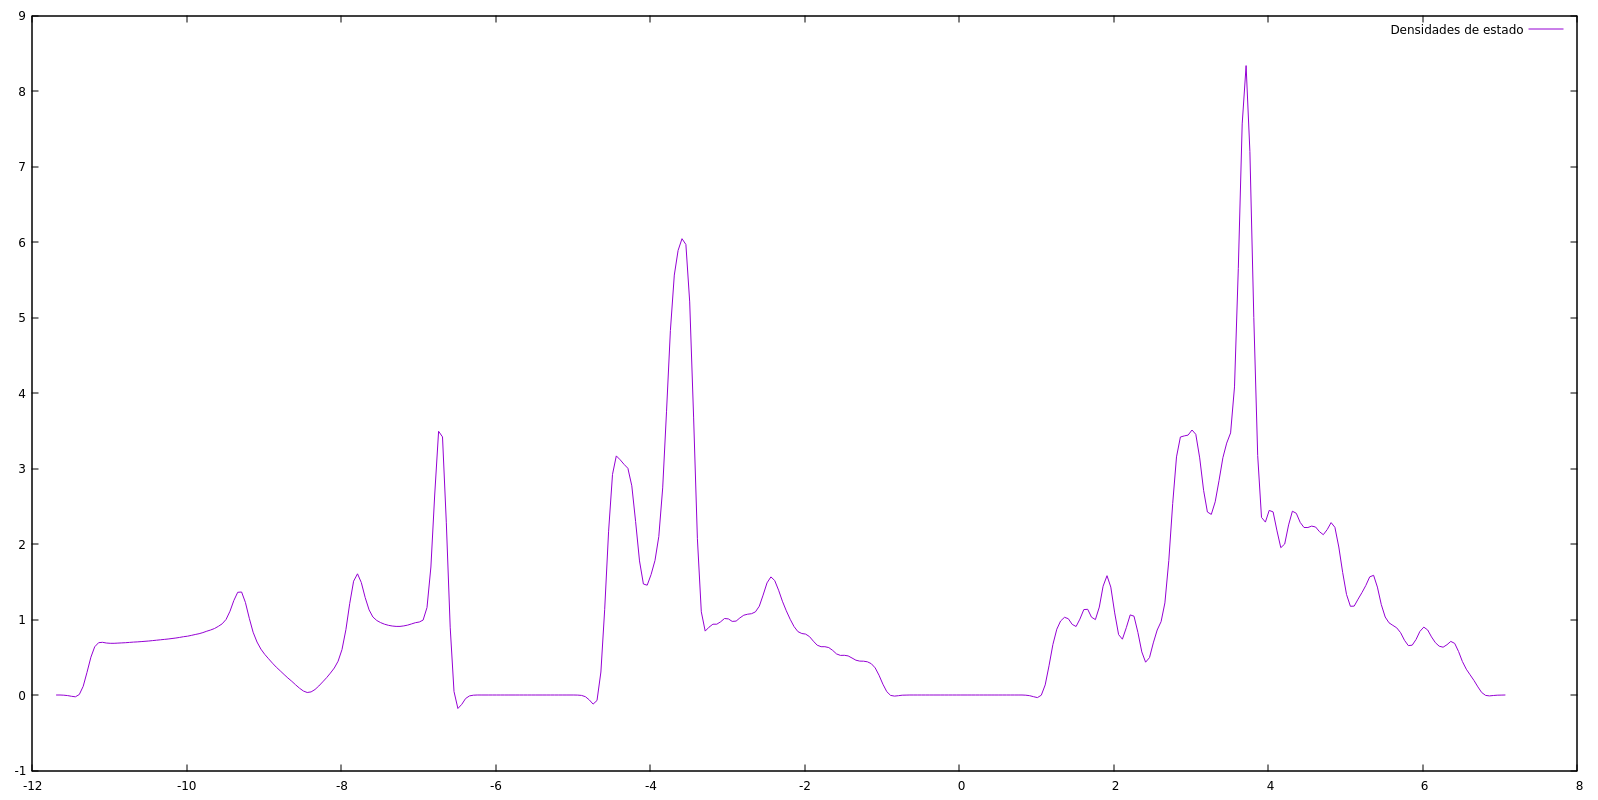
\includegraphics[scale=0.38]{images_silicano/Densidades_estado_sin_spin.png}
    \caption{Gráfica que nos muestra la densidad de estados del siliceno, sin considerar el spin.}
\end{figure}

% Densidad de estados considerando el spin [Silicano]

\newpage

\subsection{Densidad de estados considerando el spin [Silicano]}

En el siguiente apartado damos una gráfica con la densidad de estados del siliceno. Para 
ello se hizo el cálculo dentro del mismo Quantum Espresso con el módulo pw.x, primero se hizo uno cálculo 
del tipo nscf y después otro del tipo DOS. También para este momento se trabajó con la estructura
ya relajada.

\vspace{0.5cm}

\textbf{Importante: En el siguiente cálculo se consideró el spin.}

\vspace{0.5cm}

Se llegó al siguiente gráfico:

\begin{figure}[H]
    \centering
    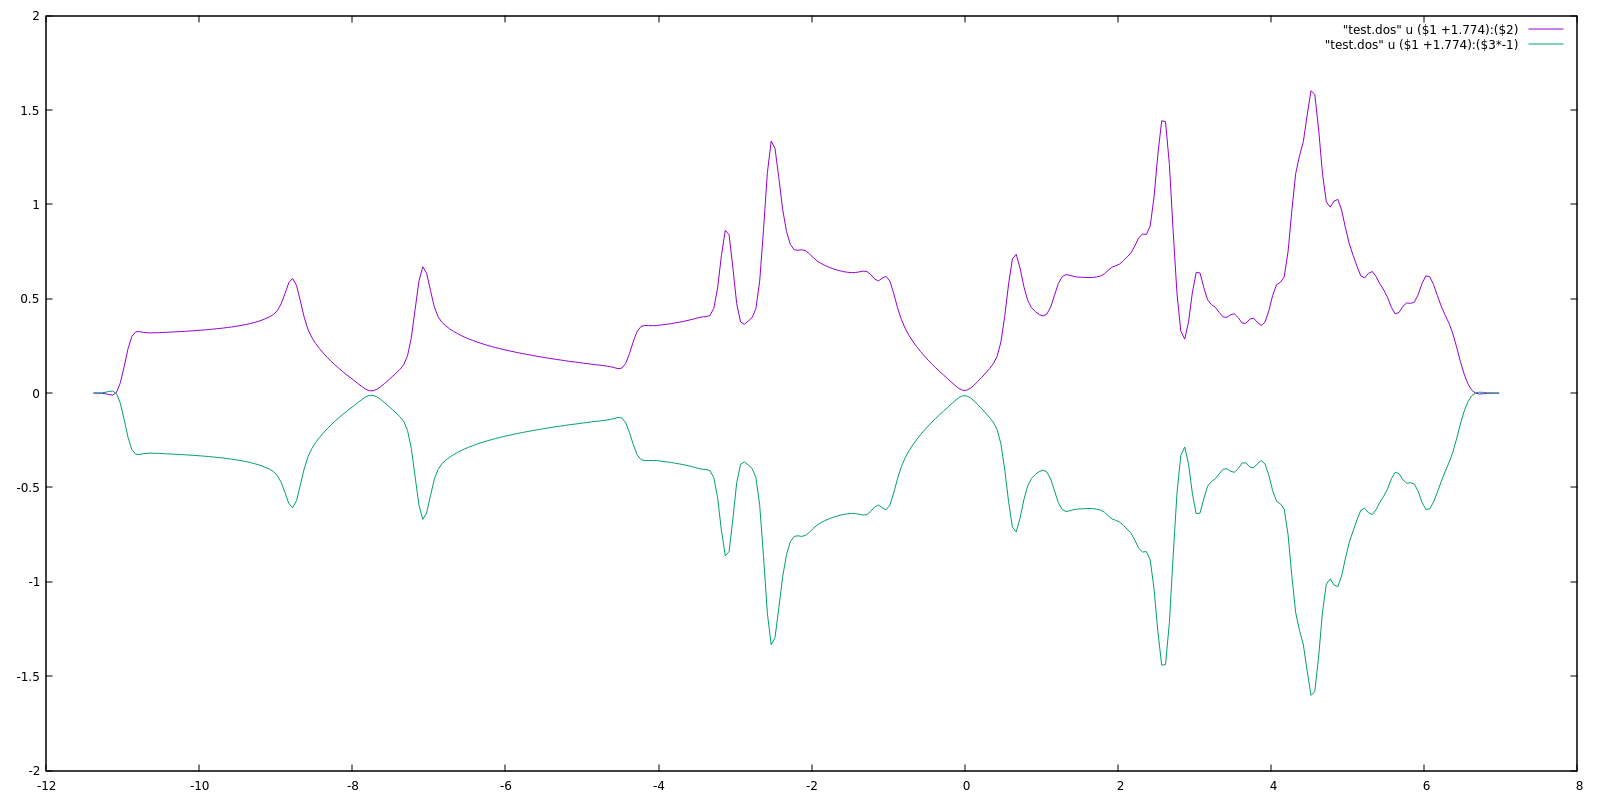
\includegraphics[scale=0.33]{images_siliceno/densidad_estados_con_spin.png}
    \caption{Gráfica que nos muestra la densidad de estados del siliceno, considerando el spin.}
\end{figure}

A continuación proporcionaremos una gráfica que nos muestra la energía por nivel orbital.

\begin{figure}[H]
    \centering
    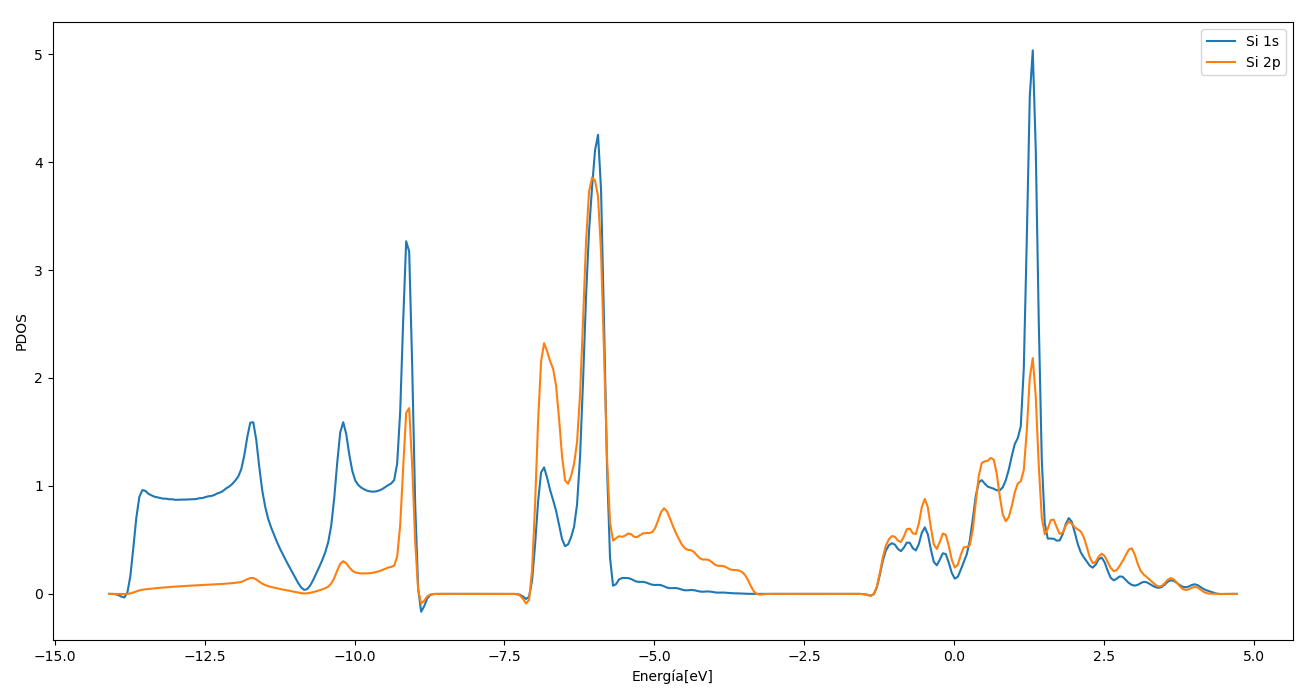
\includegraphics[scale=0.30]{images_silicano/Desnidad_por orbital.png}
    \caption{Gráfica que nos muestra la energía en los orbitales del silicano, considerando el spin.}
\end{figure}

\newpage